\chapter{API Docs}
Here are some of the API endpoints, provided by \href{https://swagger.io/}{Swagger UI}.\\
Disclaimer: This is all data within my environment, the response body can change if the environment or collections are different, but not the response structure or the response headers.
\section{api/collections}
Response body:
\begin{minted}{json}
{
  "links": [
    {
      "href": "http://127.0.0.1:8000/collections",
      "rel": "self",
      "type": "application/json",
      "title": "Collections"
    }
  ],
  "collections": [
    {
      "name": "castles",
      "title": "castles",
      "links": [
        {
          "href": "http://127.0.0.1:8000/collections/castles",
          "rel": "item",
          "type": "application/geo+json",
          "title": "castles"
        }
      ]
    }
  ]
}
\end{minted}
Response headers:
\begin{minted}{bash}
 content-length: 294 
 content-type: application/json 
 date: Fri, 06 Dec 2019 13:42:33 GMT 
 server: uvicorn 
\end{minted}
\section{api/collections/\{collection\}}
Response body:
\begin{minted}{json}
{
  "name": "castles",
  "title": "castles",
  "links": [
    {
      "href": "http://127.0.0.1:8000/collections/castles",
      "rel": "item",
      "type": "application/geo+json",
      "title": "castles"
    }
  ]
}
\end{minted}
Response headers:
\begin{minted}{bash}
 content-length: 160 
 content-type: application/json 
 date: Fri, 06 Dec 2019 13:45:05 GMT 
 server: uvicorn 
\end{minted}
\newpage
\section{api/collections/\{collection\}/items}
Response body (with only 1 feature, which means a limit of 1):
\begin{minted}{json}
{
  "type": "FeatureCollection",
  "features": [
    {
      "type": "Feature",
      "id": "N2306343684",
      "geometry": {
        "type": "Point",
        "coordinates": [
          10.749732,
          47.557561
        ]
      },
      "properties": {
        "castle_type": "stately",
        "description": "Die Schlosshöfe können kostenlos besichtigt werden. In die Schlossgebäude kommt man nur mit einem Ticket aus dem Ticketshop unten im Ort. Kein Ticketverkauf am Schloss.",
        "historic": "castle",
        "name": "Schloss Neuschwanstein   ",
        "name:ar": "(characters that LaTeX can't compile)",
        "name:be": "(characters that LaTeX can't compile)",
        "name:en": "Neuschwanstein Castle",
        "name:fr": "Château de Neuschwanstein",
        "name:ja": "(characters that LaTeX can't compile)",
        "name:ja_kana": "(characters that LaTeX can't compile)",
        "name:ru": "(characters that LaTeX can't compile)",
        "name:zh": "(characters that LaTeX can't compile)",
        "opening_hours": "Mo-Su 09:00-18:00",
        "phone": "+49 8362 93 98 80",
        "toilets:wheelchair": "yes",
        "tourism": "attraction",
        "website": "http://www.neuschwanstein.de",
        "wheelchair": "yes",
        "wikidata": "Q4152",
        "wikipedia": "de:Schloss Neuschwanstein"
      }
    }
  ],
  "bbox": [
    10.749732,
    47.557561,
    10.749732,
    47.557561
  ],
  "links": [
    {
      "href": "http://127.0.0.1:8000/collections/castles/items?limit=1",
      "rel": "self",
      "type": "application/geo+json",
      "title": "self"
    }
  ]
}
\end{minted}
Response headers:
\begin{minted}{bash}
 content-length: 1195 
 content-type: application/geo+json 
 date: Fri, 06 Dec 2019 13:46:28 GMT 
 server: uvicorn 
\end{minted}
\section{api/collections/\{collection\}/\{feature\_id\}}
Response body:
\begin{minted}{json}
{
  "type": "Feature",
  "id": "N473471590",
  "geometry": {
    "type": "Point",
    "coordinates": [
      7.488973,
      45.736946
    ]
  },
  "properties": {
    "historic": "castle",
    "name": "Castello di Fénis",
    "wikidata": "Q607126",
    "wikipedia": "it:Castello di Fénis"
  }
}
\end{minted}
Response headers:
\begin{minted}{bash}
 content-length: 219 
 content-type: application/geo+json 
 date: Fri, 06 Dec 2019 13:47:36 GMT 
 server: uvicorn 
\end{minted}
\newpage
\section{api/tiles/\{collection\}/\{zoom\}/\{x\}/\{y\}.png}
Response body:\\
\begin{figure}[H]
	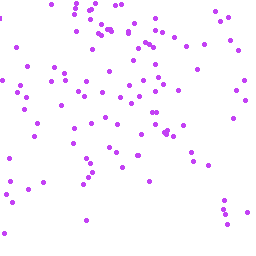
\includegraphics[width=\linewidth]{./Images/Appendices/raster_tile_response_body.png}
	\caption{A raster tile PNG response}
\end{figure}
Response headers:
\begin{minted}{bash}
 content-length: 2342 
 content-type: image/png 
 date: Fri, 06 Dec 2019 13:49:50 GMT 
 server: uvicorn 
\end{minted}
\section{api/tiles/\{collection\}/\{zoom\}/\{x\}/\{y\}/\{a\}/\{b\}.geojson}
\begin{minted}{json}
{
  "type": "FeatureCollection",
  "features": [
    {
      "type": "Feature",
      "id": "W387544802",
      "geometry": {
        "type": "Polygon",
        "coordinates": [
          [
            [
              7.406668,
              46.649168
            ],
            [
              7.406333,
              46.649
            ],
            [
              7.406405,
              46.648945
            ],
            [
              7.406735,
              46.649107
            ],
            [
              7.406668,
              46.649168
            ]
          ]
        ]
      },
      "properties": {
        "historic": "castle",
        "name": "Festi",
        "wikidata": "Q67772651"
      }
    }
  ],
  "bbox": [
    7.406668,
    46.649168,
    7.406668,
    46.649168
  ]
}
\end{minted}
Response headers:
\begin{minted}{bash}
 content-length: 348 
 content-type: application/geo+json 
 date: Fri, 06 Dec 2019 13:51:08 GMT 
 server: uvicorn 
\end{minted}
	